\documentclass[11pt]{article}
\usepackage{listings}
\usepackage{tikz}
\usepackage{alltt}
\usepackage{hyperref}
\usepackage{url}
%\usepackage{algorithm2e}
\usetikzlibrary{arrows,automata,shapes}
\tikzstyle{block} = [rectangle, draw, fill=blue!20, 
    text width=5em, text centered, rounded corners, minimum height=2em]
\tikzstyle{bt} = [rectangle, draw, fill=blue!20, 
    text width=1em, text centered, rounded corners, minimum height=2em]

\newtheorem{defn}{Definition}
\newtheorem{crit}{Criterion}
\newcommand{\true}{\mbox{\sf true}}
\newcommand{\false}{\mbox{\sf false}}

\newcommand{\handout}[5]{
  \noindent
  \begin{center}
  \framebox{
    \vbox{
      \hbox to 5.78in { {\bf Software Testing, Quality Assurance and Maintenance } \hfill #2 }
      \vspace{4mm}
      \hbox to 5.78in { {\Large \hfill #5  \hfill} }
      \vspace{2mm}
      \hbox to 5.78in { {\em #3 \hfill #4} }
    }
  }
  \end{center}
  \vspace*{4mm}
}

\newcommand{\lecture}[4]{\handout{#1}{#2}{#3}{#4}{Lecture #1}}
\topmargin 0pt
\advance \topmargin by -\headheight
\advance \topmargin by -\headsep
\textheight 8.9in
\oddsidemargin 0pt
\evensidemargin \oddsidemargin
\marginparwidth 0.5in
\textwidth 6.5in

\parindent 0in
\parskip 1.5ex
%\renewcommand{\baselinestretch}{1.25}

%\renewcommand{\baselinestretch}{1.25}
% http://gurmeet.net/2008/09/20/latex-tips-n-tricks-for-conference-papers/
\newcommand{\squishlist}{
 \begin{list}{$\bullet$}
  { \setlength{\itemsep}{0pt}
     \setlength{\parsep}{3pt}
     \setlength{\topsep}{3pt}
     \setlength{\partopsep}{0pt}
     \setlength{\leftmargin}{1.5em}
     \setlength{\labelwidth}{1em}
     \setlength{\labelsep}{0.5em} } }
\newcommand{\squishlisttwo}{
 \begin{list}{$\bullet$}
  { \setlength{\itemsep}{0pt}
     \setlength{\parsep}{0pt}
    \setlength{\topsep}{0pt}
    \setlength{\partopsep}{0pt}
    \setlength{\leftmargin}{2em}
    \setlength{\labelwidth}{1.5em}
    \setlength{\labelsep}{0.5em} } }
\newcommand{\squishend}{
  \end{list}  }
\begin{document}

\lecture{15 --- February 6, 2017}{Winter 2017}{Patrick Lam}{version 1}

\subsection*{Weak and strong mutants}
So far we've talked about requiring differences in the \emph{output}
for mutants.  We call such mutants {\bf strong mutants}.  We can relax
this by only requiring changes in the \emph{state}, which we'll call
{\bf weak mutants}.

In other words, 
\begin{itemize}
\item \emph{strong mutation}: fault must be \emph{reachable},
\emph{infect} state, and \emph{\bf propagate} to output.
\item \emph{weak mutation}: a fault which kills a mutant need only be
\emph{reachable} and \emph{infect state}.
\end{itemize}
Supposedly, experiments show that weak and strong mutation require
almost the same number of tests to satisfy them.

We restate the definition of killing mutants which we've seen before:
\begin{defn}
\emph{Strongly killing mutants}: Given a mutant
$m$ for a program $P$ and a test $t$, $t$ is said to \emph{strongly kill $m$}
iff the output of $t$ on $P$ is different from the output of $t$ on $m$.
\end{defn}

\begin{crit}
{\bf Strong Mutation Coverage} (SMC). For each mutant $m$, TR contains
a test which strongly kills $m$.
\end{crit}

{\sf What does this criterion not say?}\\[2em]
% what's the set of mutants?

\begin{defn}
\emph{Weakly killing mutants}: Given a mutant $m$ that modifies a source
location $\ell$ in program $P$ and a test $t$, $t$ is said to
\emph{weakly kill $m$} iff the \emph{state} of the execution of $P$ on
$t$ is different from the \emph{state} of the execution of $m$ on $t$,
immediately after some execution of $\ell$.
\end{defn}

{\sf How does this criterion differ from what we've tested recently in
unit tests?}\\[2em]

% behaviour, not state.

\begin{crit}
{\bf Weak Mutation Coverage} (WMC). For each mutant $m$, TR contains
a test which weakly kills $m$.
\end{crit}

Let's consider mutant $\Delta 1$ from before, i.e. we change
{\tt minVal = a} to {\tt minVal = b}. In this case:
\begin{itemize}
\item reachability: unavoidable;
\item infection: need $b \neq a$;
\item propagation: wrong {\tt minVal} needs to return to the caller;
that is, we can't execute the body of the {\tt if} statement, so we
need $b > a$.
\end{itemize}
A test case for strong mutation is therefore $a = 5, b = 7$ (return
value = \textvisiblespace, expected \textvisiblespace), and for
weak mutation $a = 7, b = 5$ (return value = \textvisiblespace, expected
\textvisiblespace).

Now consider mutant $\Delta 3$, which replaces {\tt b < a} with {\tt 
b < minVal}. This mutant is an equivalent mutant, since {\tt a = minVal}.
(The infection condition boils down to ``false''.)

Equivalence testing is, in its full generality, undecidable, but we can always
estimate.

\subsection*{Testing Programs with Mutation}
Here's a possible workflow for actually performing mutation testing.

\begin{center}
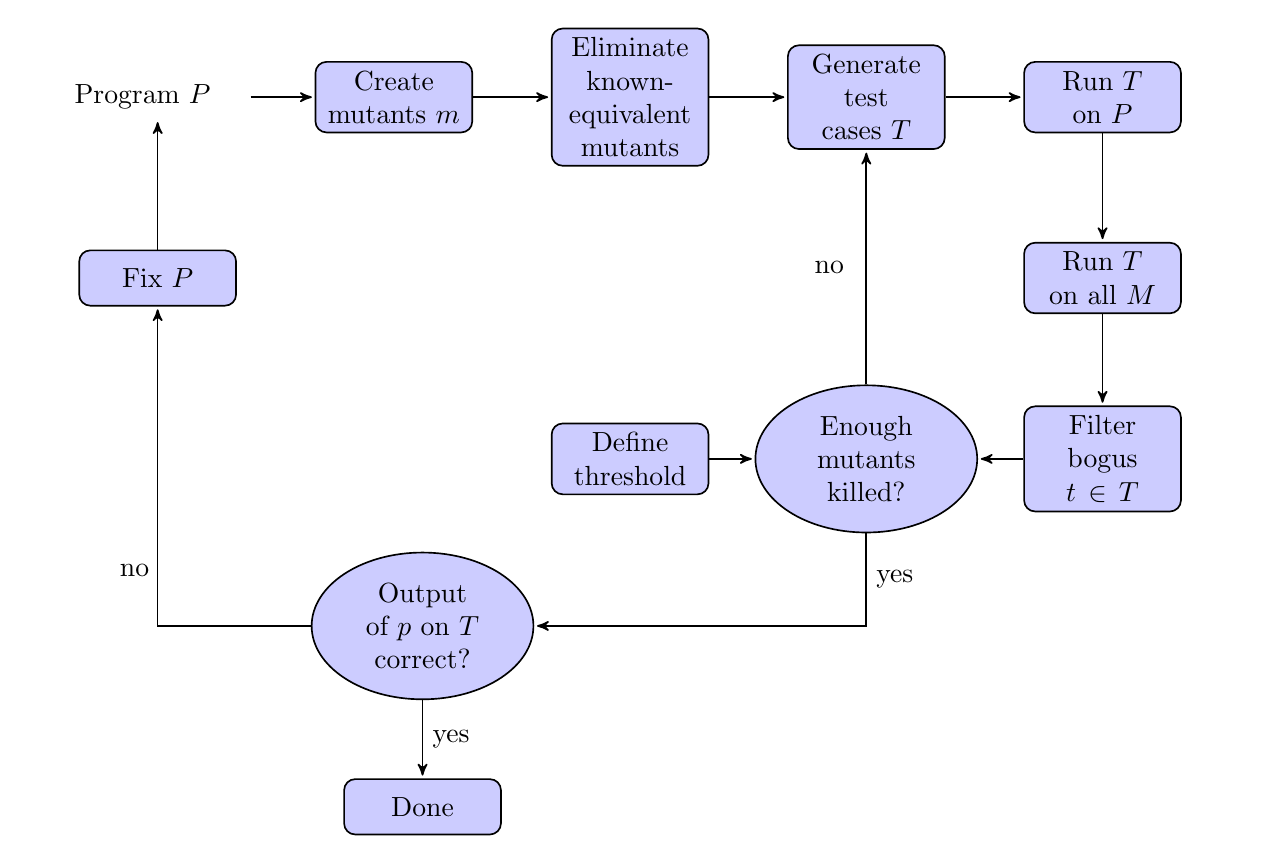
\begin{tikzpicture}[->,>=stealth',shorten >=1pt,auto,node distance=3cm,
                    text width=4em,
                    semithick,initial text=]
  \node[text width=6em] (p) {Program $P$};
  \node[block,right of=p] (create) {Create mutants $m$};
  \node[block,right of=create] (elim) {Eliminate known-equivalent mutants};
  \node[block,right of=elim] (gen) {Generate test cases $T$};
  \node[block,right of=gen] (runTonP) {Run $T$ on $P$};
  \node[block,below of=runTonP,yshift=2em] (runTonM) {Run $T$ on all $M$};
  \node[block, below of=runTonM,yshift=2em] (filter) {Filter bogus $t \in T$};
  \node[shape=ellipse, text centered, fill=blue!20, draw, text width=5em, left of=filter] (enough) {Enough mutants killed?};
  \node[block, left of=enough] (findThreshold) {Define threshold};
  \node[shape=ellipse, text centered, fill=blue!20, draw, text width=5em, below left of=enough,xshift=-10em] (correct) {Output of $p$ on $T$ correct?};
  \node[block, below of=correct,yshift=2em] (done) {Done};
  \node[block, below of=p,yshift=2em] (fixP) {Fix $P$};

  \path (p) edge node {} (create)
        (create) edge node {} (elim)
        (elim) edge node {} (gen)
        (gen) edge node {} (runTonP)
        (runTonP) edge node {} (runTonM)
        (runTonM) edge node {} (filter)
        (filter) edge node {} (enough)
        (findThreshold) edge node {} (enough)
        (correct) edge node {yes} (done)
        (fixP) edge node {} (p);
  \draw (correct) -| node[xshift=3em,yshift=2em] {no} (fixP); % no
  \draw (enough.north) -- node[xshift=2.5em] {no} (gen);
  \draw (enough) |- node[near start] {yes} (correct);
\end{tikzpicture}
\end{center}

\section*{Mutation Operators} 

We'll define a number of mutation operators, although precise
definitions are specific to a language of interest. Typical mutation
operators will encode typical programmer mistakes, e.g. by changing
relational operators or variable references; or common testing heuristics, 
e.g. fail on zero. Some mutation operators are better than others.

You can find a more exhaustive list of mutation operators in the PIT documentation: \url{http://pitest.org/quickstart/mutators/}.  How
many (intraprocedural) mutation operators can you invent for the
following code?

{ \Large
\begin{lstlisting}
int mutationTest(int a, b) { 
  int x = 3 * a, y;
  if (m > n) {
    y = -n;
  }
  else if (!(a > -b)) {
    x = a * b;
  }
  return x;
}
\end{lstlisting}
}

\paragraph{Integration Mutation.} We can go beyond mutating method bodies
by also mutating interfaces between methods, e.g.
\begin{itemize}
\item change calling method by changing actual parameter values;
\item change calling method by changing callee; or
\item change callee by changing inputs and outputs.
\end{itemize}

{
\begin{lstlisting}
class M {
  int f, g;

  void c(int x) {
    foo (x, g);
    bar (3, x);
  }

  int foo(int a, int b) {
    return a + b * f;
  }

  int bar(int a, int b) {
    return a * b;
  }
}
\end{lstlisting}
}

[Absolute value insertion, operator replacement, scalar variable replacement,
  statement replacement with crash statements\ldots]

\paragraph{Mutation for OO Programs.} One can also use some operators specific
to object-oriented programs. Most obviously, one can modify the object on
which field accesses and method calls occur.

{\small
\begin{lstlisting}
class A {
  public int x;
  Object f;
  Square s;

  void m() {
    int x;
    f = new Object();
    this.x = 5;
  }
}

class B extends A {
  int x;
}
\end{lstlisting}
}

\vspace*{-1em}
\paragraph{Exercise.} Come up with a test case to kill each of these types of
mutants.

\begin{itemize}
\item {\bf ABS}: Absolute Value Insertion\\
{\tt x = 3 * a}
$\Longrightarrow$ {\tt x = 3 * abs(a)}, {\tt x = 3 * -abs(a)}, {\tt x = 3 * failOnZero(a)};
\item {\bf ROR}: Relational Operator Replacement\\
{\tt if (m > n)} $\Longrightarrow$ {\tt if (m >= n)}, {\tt if (m < n)}, {\tt if (m <= n)}, {\tt if (m == n)}, {\tt if (m != n)}, {\tt if (false)}, {\tt if (true)}
\item {\bf UOD}: Unary Operator Deletion\\
{\tt if (!(a > -b))} $\Longrightarrow$ {\tt if (a > -b)}, {\tt if (!(a > b))}
\end{itemize}


\vspace*{-1em}
\paragraph{Summary of Syntax-Based Testing.}~\\

\begin{tabular}{l|ll}
& Program-based & Input Space/Fuzzing \\ \hline
Grammar & Programming language & Input languages / XML \\
Summary & Mutates programs / tests integration & Input space testing \\
Use Ground String? & Yes (compare outputs) & Sometimes \\
Use Valid Strings Only? & Yes (mutants must compile) & No \\
Tests & Mutants are not tests & Mutants are tests \\
Killing & Generate tests by killing & Not applicable \\
\end{tabular}

Notes: 
\squishlist
\item Program-based testing has notion of strong and weak mutants; applied
exhaustively, program-based testing subsumes many other techniques.
\item Sometimes we mutate the grammar, not strings, and get tests from the
mutated grammar.
\squishend

\paragraph{Tool support.} PIT Mutation testing tool: \url{http://pitest.org}. Mutates
your program, reruns your test suite, tells you how it went.
\end{document}
